\chapter{Sistem Tasarımı}
Sistem analizinden sonra sistem için gerekli modüller tasarlanmıştır. Tasarlanan sistemin ana işlem adımları temel olarak aşağıda listelenmiştir.
\begin{itemize}
  \item Kullanıcının anlık sensör verilerinin toplanması.
  \item Elde edilen verilerin işlenmesi.
  \item İşlenen verilerin makine öğrenmesi modelinden geçirilmesi.
  \item Sonucun kullanıcıya gösterilmesi.
\end{itemize}

\section{Yazılım Tasarımı}


Sistemin ilk aşaması çıkarım mekanizmasının yani makine öğrenmesi modelinin oluşturulmasıdır. Modelin oluşturulabilmesi için Şekil 5.1'de görülen ham sensör verilerinin işlenmesi gerekmektedir. Şekil 5.1'deki ham veriler her bir vasıta için iki farklı zaman diliminde yirmişer dakika toplanmıştır. İlk toplanan 20 dakikalık veriler makine öğrenmesi modelini eğitmek için kullanılmıştır. İkinci toplanan veriler ise makine öğrenmesi modelinin doğrulunu test etmek için kullanılmıştır. Sonuç olarak her vasıtaya ait 20 dakikalık test, 20 dakikalık eğitim veri seti oluşturulmuşur.Sensör verileri 100 Hz ile toplanmıştır.
\begin{figure}[!htbp]
\centering
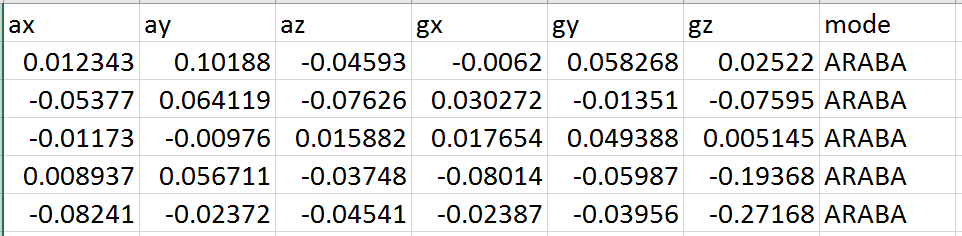
\includegraphics[scale=0.6]{projectChapters/images/rawdata.png}
\caption{Araba sınıfına ait ham sensör verisi}
\end{figure}
\newpage

İvmeölçer ve jiroskop sensörlerden toplanan bilgiler ise aşağıdaki gibidir.
\begin{itemize}
  \item AX: İvmeölçer X-Koordinatı (Accelerometer X-Coordinate)
  \item AY: İvmeölçer Y-Koordinatı (Accelerometer Y-Coordinate)
  \item AZ: İvmeölçer Z-Koordinatı (Accelerometer Z-Coordinate)
  \\
  \item GX: Jiroskop X-Koordinatı (Gyroscope X-Coordinate)
  \item GY: Jiroskop Y-Koordinatı (Gyroscope Y-Coordinate)
  \item GZ: Jiroskop Z-Koordinatı (Gyroscope Z-Coordinate)
\end{itemize}

Elde edilen eğitim veri seti ve test veri seti özellik çıkarımı işleminden geçirilmiştir. Tablo 5.1'de görülen toplan 19 istatistiksel özellik her bir eksen için çıkarılmıştır. Altı farklı eksen için toplam 114 özellik çıkarılmıştır. Özellik çıkarımı 20 saniye, 40 saniye ve 60 saniye olmak üzere 3 farklı pencere aralığı için gerçekleştirilmiştir. Özellik çıkarımı sonucunda 
\begin{itemize}
  \item 20 saniye pencere aralığına sahip test ve eğitim veri seti
  \item 40 saniye pencere aralığına sahip test ve eğitim veri seti
  \item 60 saniye pencere aralığına sahip test ve eğitim veri seti
\end{itemize}
olmak üzere toplamda 6 farklı veri seti elde edilmiştir.

%Projede girdi olarak kullanıcının anlık sensör verileri kullanılmaktadır. Projede kullanılan sensörler daha öncede belirtildiği üzere jiroskop ve ivmeölçerdir. Bu sensörlerden veriler toplanırken CoreMotion kütüphanesinden faydalanılmıştır. Sensörlerden belirli pencere boyutunda, 40 saniye, veri toplanır ve toplanan bu veriler bir sonraki aşamaya gönderilir. Sensörlerden toplanan bilgiler ise aşağıdaki gibidir.

%Her bir sensörün 3 eksendeki değerleri elde edilip kaydedilmektedir. Bu veriler, makine öğrenmesi modelinde kullanılabilecek durumda olmadığı için ilk olarak özellik çıkarımı işleminden geçirilirler. Her bir eksen için özellik çıkarımı işlemi uygulanır ve yeni bir veri seti elde edilir. Elde edilen bu yeni veri seti bir sonraki aşama olan makine öğrenmesi modeline girdi olarak kullanılmaktadır.

\begin{table}[!htbp]
\centering
\caption{Özellik çıkarımı için kullanılan özellikler}
\label{my-label}
\begin{tabular}{|l|l|}
\hline
\multicolumn{1}{|c|}{\textbf{Özellik}} & \multicolumn{1}{c|}{\textbf{Açıklama}}                        \\ \hline
Minimum Reduction                      & Ardışık veriler arasındaki minimum azalma miktarı             \\ \hline
Maximum Reduction                      & Ardışık veriler arasındaki maksimum azalma miktarı            \\ \hline
Minimum Increase                       & Ardışık veriler arasındaki minimum artma miktarı              \\ \hline
Maximum Increase                       & Ardışık veriler arasındaki maksimum artma miktarı             \\ \hline
Minimum Value                          & Veriler içerisindeki en küçük değer                           \\ \hline
Maximum Value                          & Veriler içerisindeki en büyük değer                           \\ \hline
Range                                  & Veriler içerisindeki maksimum ile minimum değer farkı         \\ \hline
Arithmetic Mean                        & Verilerin aritmetik ortalaması                                \\ \hline
Square mean                            & Verilerin karelerinin ortalaması                              \\ \hline
Harmonic Mean                          & Verilerin armonik ortalaması                                  \\ \hline
Geometric mean                         & Verilerin geometrik ortalaması                                \\ \hline
Quadratic mean                         & Verilerin kuadratik ortalaması                                \\ \hline
Median                                 & Veri içerisindeki orta değer                                  \\ \hline
Standard Deviation                     & Verilerin standart sapması                                    \\ \hline
Variance                               & Verilerin varyansı                                            \\ \hline
Coefficient of Variation               & Verilerin varyasyon katsayısı                                 \\ \hline
Kurtosis                               & Verilerin dağılımını gösteren çan eğrisinin basıklık derecesi \\ \hline
Skewness                               & Verilerin dağılımın ortalamaya göre simetrisizliği            \\ \hline
Interquartile Range                    & Verilerin çeyrekler açıklığı                                  \\ \hline
\end{tabular}
\end{table}

Özellik çıkarımı işlemi yapıldıktan sonra özellik seçimi işlemi gerçekleştirilmiştir. Özellik seçimi, sınıflandırma işlemi için kullanılacak özelliklerin belirlenmesi aşamasında, tüm özellik kümesi sütunlarından bağımlı değişkenle olan ilişkiyi açıklamada, ilgisiz sütunların elenmesi ve açıklayıcı gücü yüksek sütun alt kümelerinin belirlenmesi işlemidir. Toplam 114 olan özellik sayısı bu aşamada düşürülmüştür. Özellik seçimi alogirtmaları eğitim veri seti üzerinde çalıştırılır. Algoritmalar sonuç olarak kullanılması gereken özelliklerin listesini sunar. Listelenen özellikler dışındaki özellikler hem eğitim hem de test veri setinden çıkarılarak yeni veri setleri elde edilir.

\begin{itemize}
  \item 20 saniye pencere aralığı için 23 özellik seçilmiştir.
  \item 40 saniye pencere aralığı için 20 özellik seçilmiştir.
  \item 60 saniye pencere aralığı için 15 özellik seçilmiştir.
\end{itemize}

Özellik seçimi yapıldıktan sonra elde edilen yeni eğitim veri setleri makine öğrenmesi algoritmalarından geçirilmiştir. Aşağıda belirtilen 4 farklı makine öğrenmesi algortiması kullanılmıştır.
\begin{itemize}
  \item Naive-Bayes
  \item KNN
  \item J48
  \item Random Forest
\end{itemize}
%Projede özellik çıkarımı için kullanılan istatistiksel özelliker aşağıdaki tabloda gösterilmektedir. Her bir eksen için aşağıda belirtilen 19 özelliğin tamamı çıkarılmamaktadır. Belirli eksenler için ihtiyaç duyulan bazı özellikler kullanılır. Bu işleme özellik seçimi adı verilir. Özellik seçimi sayesinde, tahmin işleminde hiçbir etkisi olmayan özelliklerin elenmesi sağlanır. Aynı zamanda veri setinin boyutu azaltılmış olur. Özellik seçimi uygulama içerisinde gerçekleşmez. 

%Her bir eksen için hangi özelliklerin çıkarılacağı daha önceden belirlenmektedir. Bu işlem için açık kaynak kodlu bir yazılım olan Weka kullanılmıştır. Özellik seçimi işlemi iki aşamada gerçekleşmektedir. İlk olarak makine öğrenmesi modeli oluşturmak için kullanılan ve daha önceden oluşturulmuş eğitim veri seti  üzerinde CfsSubsetEval algoritması çalıştırılır. Bu algoritma ile özelliklerin bir alt kümesi belirlenir. Bu alt kümeler arsından en iyisinin belirlenmesi için BestFirst algoritması çalıştırılır. Sonuç olarak girdi olarak verilen veri setinin modellenmesinde kullanılması gereken özellikler listelenir. Bu işlem ile belirlenen özellikler uygulama içerisindeki veri setinde kullanılır.

%Elde edilen yeni veri seti makine öğrenmesi modelinden geçirilir. Makine öğrenmesi modeli bir önceki adımda yani özellik seçimi adımında olduğu gibi uygulama içerisinde değil Weka üzerinde daha önceden oluşturulur. 
%Eğitim veri seti özellik çıkarımı ve özellik seçimi işleminden geçirildikten sonra belirli makine öğrenmesi algoritmalarından geçirilir. Bu algoritmalardan en iyi doğruluk oranını veren algoritmanın oluşturduğu model uygulamada kullanılır.



Naive-Bayes algoritması eğitim verisi üzerinden öğrenme işlemini gerçekleştirir ve en yüksek orandaki örneğini sınıfa dahil eder. Algoritma verinin hangi sınıfa ait olduğunu belirlemek için Bayes Teoremi olasılığını hesaplar.
\\
KNN algoritmasında (Şekil 5.2) sınıflandırılacak olan yeni örneğe eğitim setinden en yakın mesafedeki k tane örneğe bakılır ve bu k örnek çoğunluk olarak hangi sınıfa dâhil edilmiş ise yeni örnek de o sınıfa dâhil edilir. Mesafe hesabı olarak ise yaygın bilinen  Manhattan uzaklık ölçütü, Öklid uzaklık ölçütü ve Minkowski uzaklık ölçütü formüllerinden bir tanesi kullanılır.
\begin{figure}[!htbp]
\centering
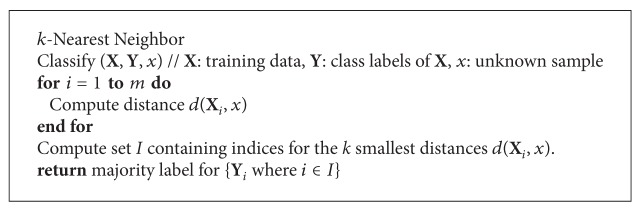
\includegraphics[width=\textwidth]{projectChapters/images/Pseudocode-for-KNN-classification.jpeg}
\caption{KNN algoritmasına ait sözde kod}
\end{figure}

J48 algoritması (Şekil 5.3) bilgi entropi kavramı kullanarak bir eğitim setinden karar ağacı inşa eder. Ağacın her bir düğümünde J48, alt kümelerdeki zenginleştirilmiş verinin niteliğini seçer. Bölünme ölçütü normalize bilgi kazancıdır. En yüksek normalize bilgi kazancına sahip nitelik karar için seçilir. Sonrasında J48 algoritması daha küçük alt listelerden çekilir.


\begin{figure}[!htbp]
\centering
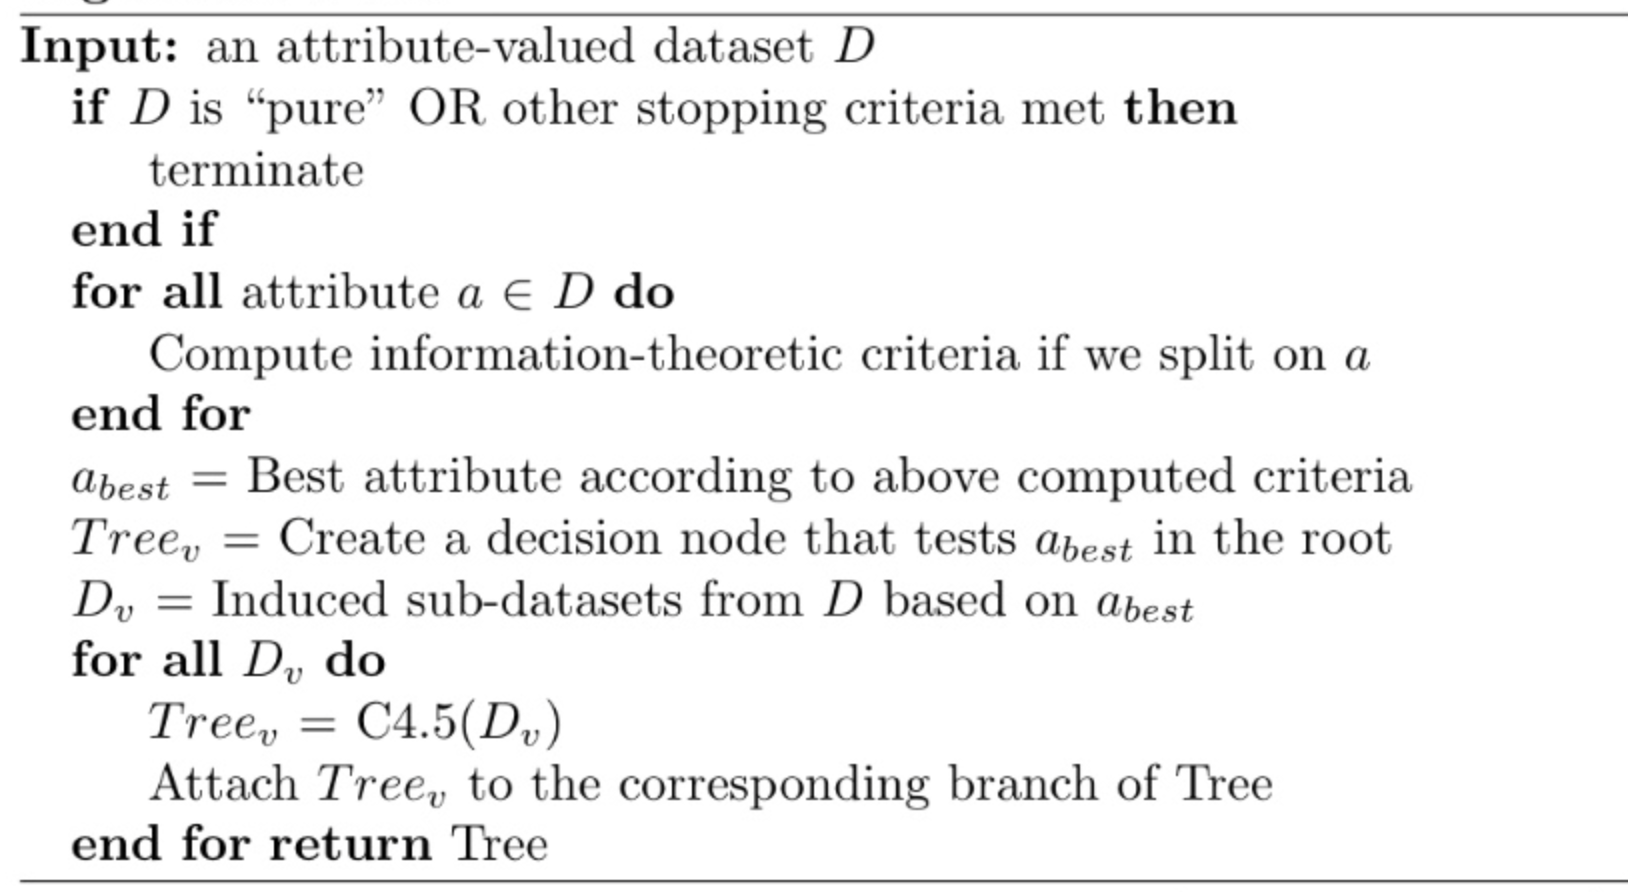
\includegraphics[width=\textwidth]{projectChapters/images/j48pscode.png}
\caption{J48 algoritmasına ait sözde kod}
\end{figure}

\begin{figure}[!htbp]
\centering
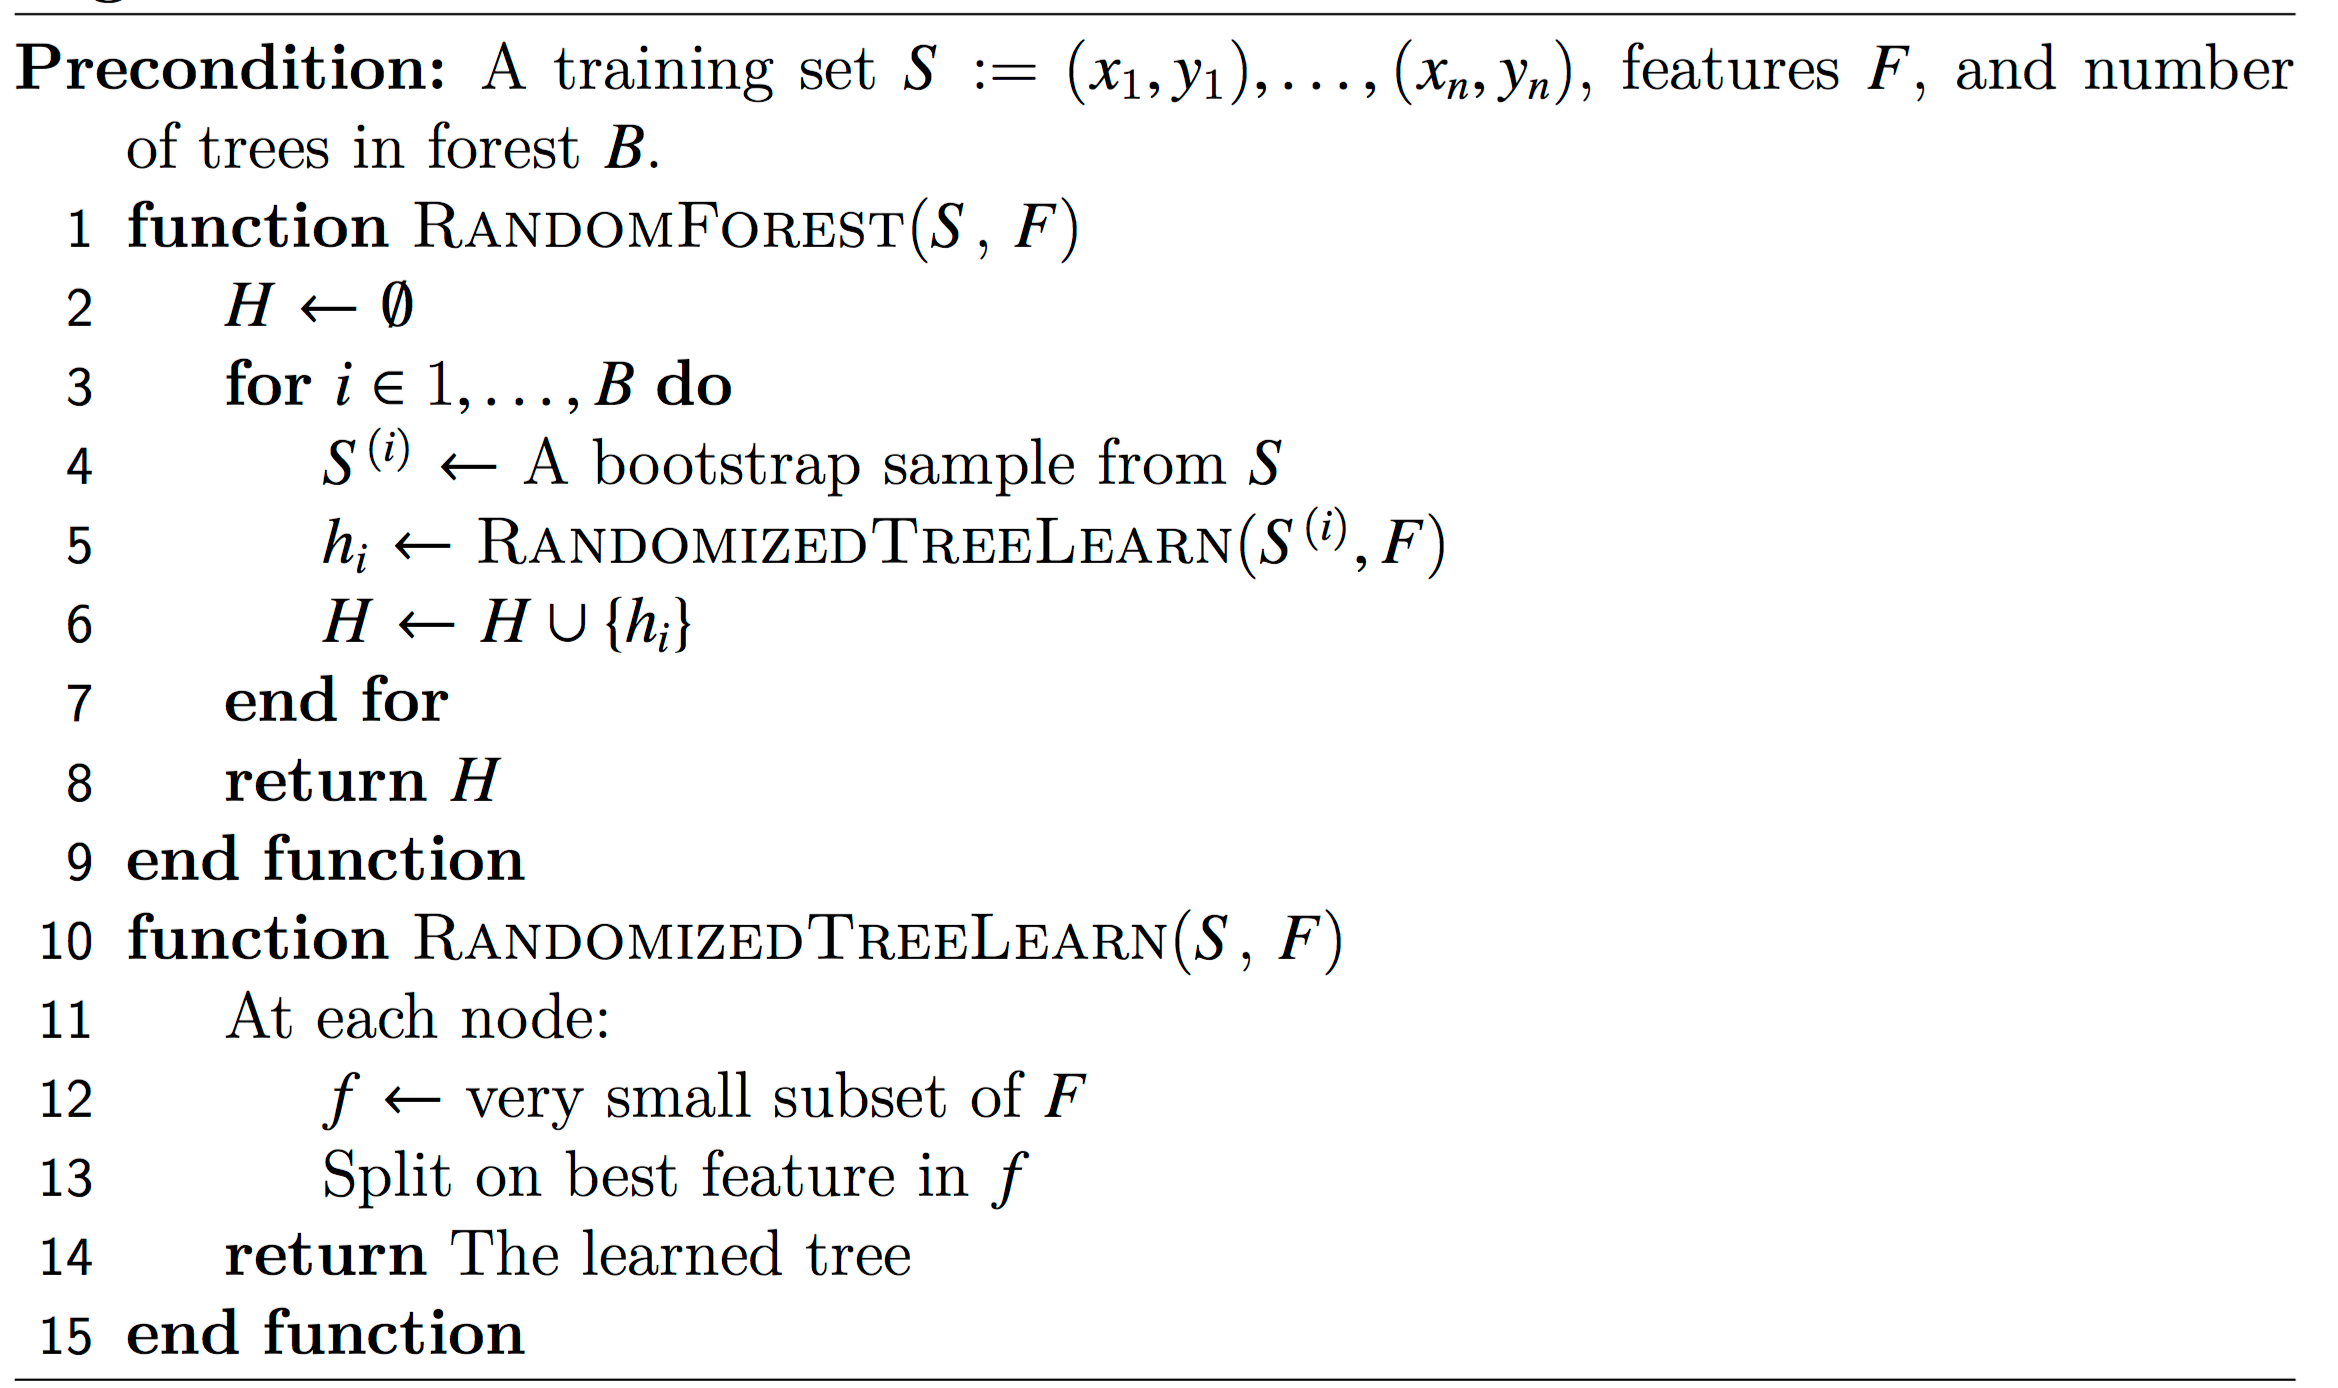
\includegraphics[width=\textwidth]{projectChapters/images/randomForest.png}
\caption{Random Forest algoritmasına ait sözde kod}
\end{figure}

Random Forest algoritmasında (Şekil 5.4) amaç tek bir karar ağacı üretmek yerine her biri farklı eğitim kümelerinde eğitilmiş olan çok sayıda çok değişkenli ağacın kararlarını birleştirmektir. Farklı eğitim kümeleri oluştururken ön yükleme ve rastgele özellik seçimi kullanılır. Çok değişkenli karar ağaçları oluşturulurken CART algoritması kullanılır. Her seviyedeki özniteliği belirlerken önce bütün ağaçlarda hesaplamalar yapılarak nitelik belirlenir, ardından bütün ağaçlardaki nitelikler birleştirilerek en fazla kullanılan öznitelik seçilir. Seçilen nitelik ağaca dahil edilerek diğer seviyelerde aynı işlemler tekrarlanır.


20 saniye, 40 saniye ve 60 saniye pencere aralığına sahip eğitim veri setlerinin yukarıda belirtilen makine öğrenmesi algoritmalarından geçirilmesi sonucu elde edilen doğruluk değeleri Tablo 5.2'deki gibidir. Tablo 5.2 incelendiğinde 60 saniye pencere aralığı oldukça düşük doğruluk oranına sahiptir. 20 saniye ve 40 saniye pencere aralığı daha iyi sonuç üretmektedir. En iyi sonuç 20 saniye pencere aralığında J48 algoritmasından alınmaktadır.
\begin{table}[!htbp]
\centering
\caption{Eğitim veri setlerinin doğruluk değerleri}
\label{my-label}
\begin{tabular}{|l|l|l|l|}
\hline
              & 20 Saniye  & 40 Saniye  & 60 Saniye  \\ \hline
Naive Bayes   & \% 54.4492 & \% 55.819  & \% 56.9079 \\ \hline
KNN           & \% 49.8941 & \% 51.0776 & \% 54.6053 \\ \hline
J48           & \% 65.1483 & \% 61.2069 & \% 54.2763 \\ \hline
Random Forest & \% 60.5932 & \% 60.9914 & \% 58.2237 \\ \hline
\end{tabular}
\end{table}
\newpage
Tablo 5.2'de belirtilen doğruluk değerlerine ait karmaşıklık matrisleri; Naive Bayes algoritması için Şekil 5.5'de, KNN algoritması için Şekil 5.6'da, J48 algoritması için Şekil 5.7'de ve son olarak Random Forest algortması için Şekil 5.8'de gösterilmiştir.

\begin{figure}[!h]
\centering
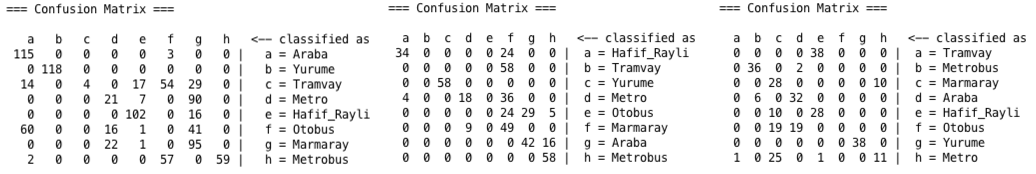
\includegraphics[width=\textwidth]{projectChapters/images/NB.png}
\caption{Naive Bayes algoritmasının sırasıyla 20 - 40 - 60 saniye için karmaşıklık matrisi}
\end{figure}

\begin{figure}[!h]
\centering
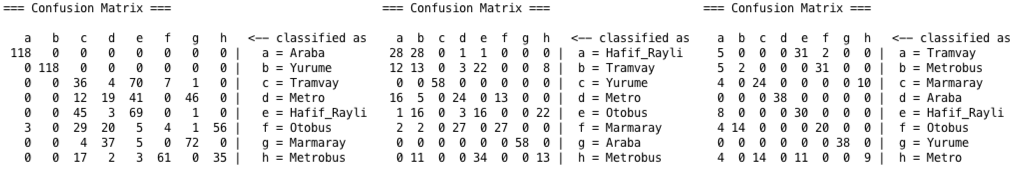
\includegraphics[width=\textwidth]{projectChapters/images/KNN.png}
\caption{KNN algoritmasının sırasıyla 20 - 40 - 60 saniye için karmaşıklık matrisi}
\end{figure}

\begin{figure}[!h]
\centering
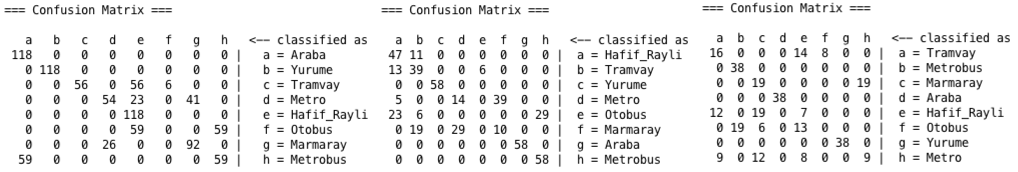
\includegraphics[width=\textwidth]{projectChapters/images/J48.png}
\caption{J48 algoritmasının sırasıyla 20 - 40 - 60 saniye için karmaşıklık matrisi}
\end{figure}

\begin{figure}[!h]
\centering
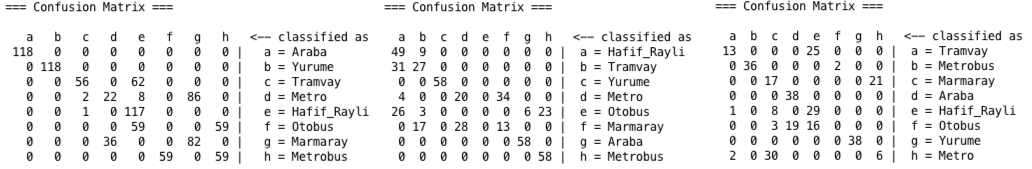
\includegraphics[width=\textwidth]{projectChapters/images/RF.png}
\caption{Random Forest algoritmasının sırasıyla 20 - 40 - 60 saniye için karmaşıklık matrisi}
\end{figure}


Karmaşıklık matrisleri incelendiğinde Metro - Marmaray ve Otobüs - Metrobüs ikililerinin birbiri ile çok fazla karıştırıldığı görülmektedir. Bu ikililer tek bir sınıf altında birleştirildiğinde doğruluk değerleri Tablo 5.3'deki gibi olmaktadır.

%\begin{table}[!h]
%\centering
%\caption{Sınıfların birleştirilmesiyle elde edilen doğruluk değerleri}
%\label{my-label}
%\begin{tabular}{|l|l|l|}
%\hline
%              & 20 Saniye  & 40 Saniye  \\ \hline
%Naive Bayes   & \% 74.7881 & \% 73.7069 \\ \hline
%KNN           & \% 73.6229 & \% 77.8017 \\ \hline
%J48           & \% 85.6992 & \% 67.2414 \\ \hline
%Random Forest & \% 85.5127 & \% 85.3448 \\ \hline
%\end{tabular}
%\end{table}


\begin{table}[]
\centering
\caption{Sınıfların birleştirilmesiyle elde edilen doğruluk değerleri}
\label{my-label}
\begin{tabular}{|l|l|l|l|}
\hline
              & 20 Saniye  & 40 Saniye  & 60 Saniye  \\ \hline
Naive Bayes   & \% 74.7881 & \% 73.7069 & \% 78.3826 \\ \hline
KNN           & \% 73.6229 & \% 77.8017 & \% 79.2763 \\ \hline
J48           & \% 85.6992 & \% 67.2414 & \% 75      \\ \hline
Random Forest & \% 85.5127 & \% 85.3448 & \% 81.9079 \\ \hline
\end{tabular}
\end{table}

Tablo 5.3'de belirtilen doğruluk değerlerinin karmaşıklık matrisleri; Naive Bayes algoritması için Şekil 5.9'de, KNN algoritması için Şekil 5.10'da, J48 algoritması için Şekil 5.11'de ve son olarak Random Forest algortması için Şekil 5.12'de gösterilmiştir.

\begin{figure}[!h]
\centering
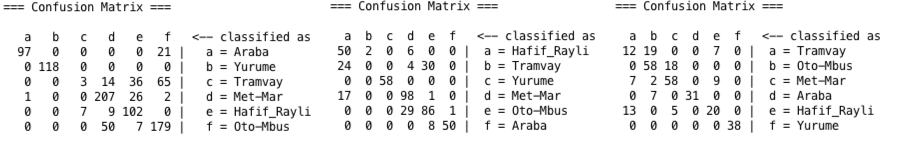
\includegraphics[width=\textwidth]{projectChapters/images/NB_2_2.png}
\caption{Naive Bayes algoritmasının sırasıyla 20 - 40 - 60 saniye için karmaşıklık matrisi}
\end{figure}

\begin{figure}[!h]
\centering
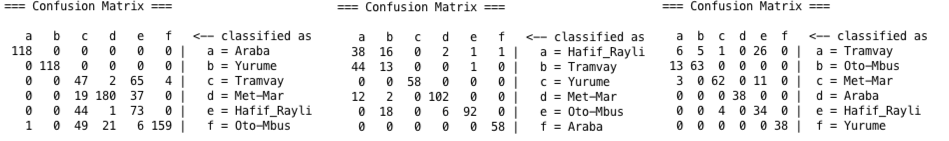
\includegraphics[width=\textwidth]{projectChapters/images/KNN_2_2.png}
\caption{KNN algoritmasının sırasıyla 20 - 40 - 60 saniye için karmaşıklık matrisi}
\end{figure}

\begin{figure}[!h]
\centering
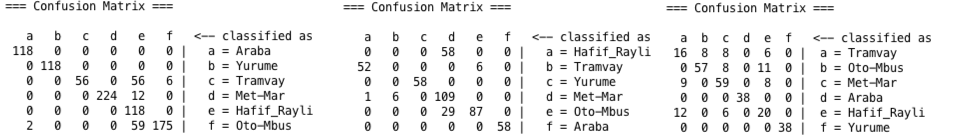
\includegraphics[width=\textwidth]{projectChapters/images/J48_2_2.png}
\caption{J48 algoritmasının sırasıyla 20 - 40 - 60 saniye için karmaşıklık matrisi}
\end{figure}

\begin{figure}[!h]
\centering
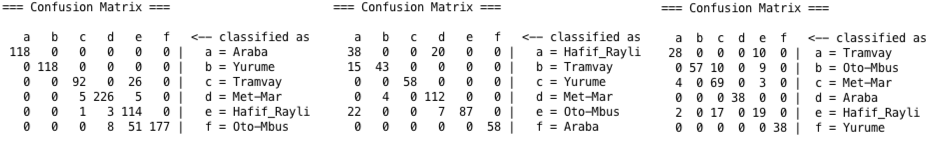
\includegraphics[width=\textwidth]{projectChapters/images/RF_2_2.png}
\caption{Random Forest algoritmasının sırasıyla 20 - 40 - 60 saniye için karmaşıklık matrisi}
\end{figure}
Metro-Marmaray ikilisi Met-Mar şeklinde, Otobüs-Metrobüs ikilisi ise Oto-Mbus şeklinde temsil edilmiştir.

Sonuçlar incelendiğinde en uygun model J48 algoritması tarafından oluşturulan ve 20 saniye pencere aralığı içeren makine öğrenmesi modeli olduğu görülmüştür. Sistemin çıkarım mekanizması olarak Şekil 5.13'deki model tercih edilmiştir.
\begin{figure}[!h]
\centering
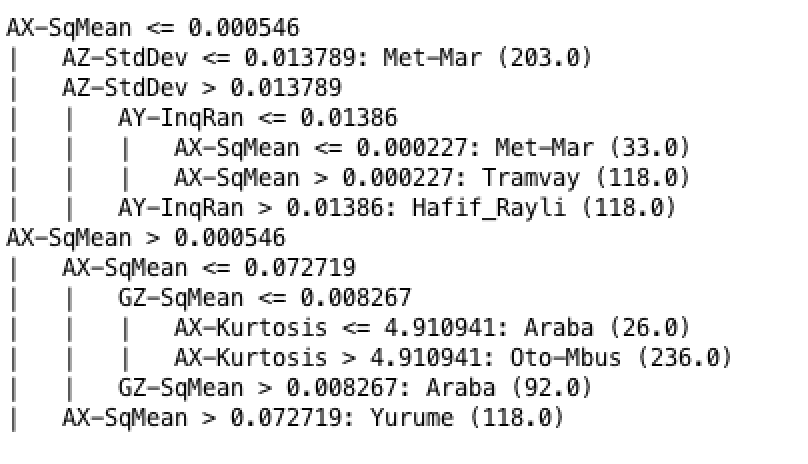
\includegraphics[scale = 0.8]{projectChapters/images/j48model.png}
\caption{Sistemin J48 algoritması tarafından oluşturulan makine öğrenmesi modeli}
\end{figure}

Kullanıcının akıllı telefonuna ait 20 saniyelik sensör verisi Şekil 5.13'de belirtilen makine öğrenmesi modelinden geçirilmeden önce sözde kodu Şekil 5.14'de görülen gürültü önleyici bir filtreden geçirilerek aykırı verilerin temizlenmesi sağlanır. 
\begin{figure}[!h]
\centering
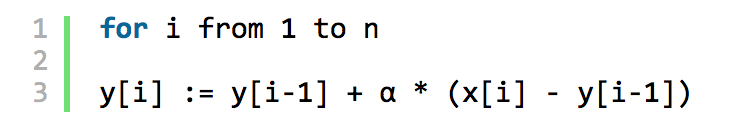
\includegraphics[scale = 0.8]{projectChapters/images/lowPassFilter.png}
\caption{Alçak geçirgen filtre sözde kodu}
\end{figure}

Her 20 saniye de bir toplanan filtrelenmiş sensör verileri makine öğrenmesi modelinden geçirilir. Elde edilen zaman ve ulaşım türü bilgileri geçici olarak saklanır. Veri toplama işlemi durdurulduğunda depolanan veriler incelenerek farklı zamanlardaki ardışık iki yürüme işlemi arasında yer alan  taşıt bilgilerinden en fazla olan bulunur; aradaki tüm taşıt bilgileri bulunan taşıt bilgisi ile etiketlenir. Elde edilen veriler işlenerek herbir zaman aralığında hangi vasıta ile ne kadar süre seyehat edildiği veritabanında saklanır.


\section{Veritabanı Tasarımı}
Projede toplanan verilerin saklanması için veritabanı yapısı kullanılmıştır. Kullanılan veritabanı ise CoreData yapısıdır. Veritabanı iki tablodan oluşmaktadır.


\begin{table}[!htbp]
\centering
\caption{Sensor verileri tablosu}
\label{myl}
\begin{tabular}{|l|l|l|l|l|l|l|}
\hline
AX & AY & AZ & GX & GY & GZ & Mode \\ \hline
\end{tabular}
\end{table}

Tablo 7.4'de Ax-Ay-Az sütunları ivmeölçerin o anki x-y-z koordinatlarındaki değerlerini tutmaktadır. Gx-Gy-Gz sütunları jiroskopun o anki x-y-z koordinatlarındaki değerlerini tutmaktadır. Mode sütununda ise verilerin kaydının yapıldığı ulaşım türü bilgisi tutulmaktadır.

\begin{table}[!htbp]
\centering
\caption{Ulaşım türü tablosu}
\begin{tabular}{|l|l|l|}
\hline
Tarih & Saat & Mode \\ \hline
\end{tabular}
\end{table}

Tablo 7.5'de uygulama tarafından tahmin edilen ulaşım türü aşağıdaki tabloya kayıt edilir.
Tarih ve saat sütunlarında ulaşım türünün belirlendiği tarih ve saat bilgisi tutulur. Mode sütununda kullanıcının seyehat ettiği vasıta ismi yazmaktadır.

\begin{table}[!htbp]
\centering
\caption{Ulaşım türü - süre tablosu}
\label{my-label}
\begin{tabular}{|l|l|}
\hline
Süre & Mode \\ \hline
\end{tabular}
\end{table}

Tablo 7.6'da görülen veritabanı tablosunda belirli zaman aralıklarında hangi ulaşım türü ile ne kadar süre seyehat edildiği bilgisi tutulmaktadır. Süre sütununda ulaşım türünün süresi, mode sütununda ise ulaşım türü bilgisi bulunmaktadır.

\section{Girdi Çıktı Tasarımı}
Sistemde girdi bilgisi olarak sensör verileri alınmaktadır. Kullanıcı bireysel olarak herhangi bir bilgi girmemektedir.

Sistemde çıktı bilgisi olarak kullanıcının o anki ulaşım türü verilmektedir. Çıktı araba, otobüs, metrobüs, metro, marmaray, hafif raylı ve tramvay vasıtalarından herhangi bir tanesidir.

